
%% bare_conf.tex 
%% V1.2
%% 2002/11/18
%% by Michael Shell
%% mshell@ece.gatech.edu
%% 
%% NOTE: This text file uses UNIX line feed conventions. When (human)
%% reading this file on other platforms, you may have to use a text
%% editor that can handle lines terminated by the UNIX line feed
%% character (0x0A).
%% 
%% This is a skeleton file demonstrating the use of IEEEtran.cls 
%% (requires IEEEtran.cls version 1.6b or later) with an IEEE conference paper.
%% 
%% Support sites:
%% http://www.ieee.org
%% and/or
%% http://www.ctan.org/tex-archive/macros/latex/contrib/supported/IEEEtran/ 
%%
%% This code is offered as-is - no warranty - user assumes all risk.
%% Free to use, distribute and modify.

% *** Authors should verify (and, if needed, correct) their LaTeX system  ***
% *** with the testflow diagnostic prior to trusting their LaTeX platform ***
% *** with production work. IEEE's font choices can trigger bugs that do  ***
% *** not appear when using other class files.                            ***
% Testflow can be obtained at:
% http://www.ctan.org/tex-archive/macros/latex/contrib/supported/IEEEtran/testflow


% Note that the a4paper option is mainly intended so that authors in
% countries using A4 can easily print to A4 and see how their papers will
% look in print. Authors are encouraged to use U.S. letter paper when 
% submitting to IEEE. Use the testflow package mentioned above to verify
% correct handling of both paper sizes by the author's LaTeX system.
%
% Also note that the "draftcls" or "draftclsnofoot", not "draft", option
% should be used if it is desired that the figures are to be displayed in
% draft mode.
%
% This paper can be formatted using the peerreviewca
% (instead of conference) mode.
\documentclass[conference]{IEEEtran}

% some very useful LaTeX packages include:

\usepackage{cite}      % Written by Donald Arseneau
                        % V1.6 and later of IEEEtran pre-defines the format
                        % of the cite.sty package \cite{} output to follow
                        % that of IEEE. Loading the cite package will
                        % result in citation numbers being automatically
                        % sorted and properly "ranged". i.e.,
                        % [1], [9], [2], [7], [5], [6]
                        % (without using cite.sty)
                        % will become:
                        % [1], [2], [5]--[7], [9] (using cite.sty)
                        % cite.sty's \cite will automatically add leading
                        % space, if needed. Use cite.sty's noadjust option
                        % (cite.sty V3.8 and later) if you want to turn this
                        % off. cite.sty is already installed on most LaTeX
                        % systems. The latest version can be obtained at:
                        % http://www.ctan.org/tex-archive/macros/latex/contrib/supported/cite/

%\usepackage{graphicx}  % Written by David Carlisle and Sebastian Rahtz
                        % Required if you want graphics, photos, etc.
                        % graphicx.sty is already installed on most LaTeX
                        % systems. The latest version and documentation can
                        % be obtained at:
                        % http://www.ctan.org/tex-archive/macros/latex/required/graphics/
                        % Another good source of documentation is "Using
                        % Imported Graphics in LaTeX2e" by Keith Reckdahl
                        % which can be found as esplatex.ps and epslatex.pdf
                        % at: http://www.ctan.org/tex-archive/info/
% NOTE: for dual use with latex and pdflatex, instead load graphicx like:
\ifx\pdfoutput\undefined
\usepackage{graphicx}
\else
\usepackage[pdftex]{graphicx}
\fi

% However, be warned that pdflatex will require graphics to be in PDF
% (not EPS) format and will preclude the use of PostScript based LaTeX
% packages such as psfrag.sty and pstricks.sty. IEEE conferences typically
% allow PDF graphics (and hence pdfLaTeX). However, IEEE journals do not
% (yet) allow image formats other than EPS or TIFF. Therefore, authors of
% journal papers should use traditional LaTeX with EPS graphics.
%
% The path(s) to the graphics files can also be declared: e.g.,
% \graphicspath{{../eps/}{../ps/}}
% if the graphics files are not located in the same directory as the
% .tex file. This can be done in each branch of the conditional above
% (after graphicx is loaded) to handle the EPS and PDF cases separately.
% In this way, full path information will not have to be specified in
% each \includegraphics command.
%
% Note that, when switching from latex to pdflatex and vice-versa, the new
% compiler will have to be run twice to clear some warnings.


%\usepackage{psfrag}    % Written by Craig Barratt, Michael C. Grant,
                        % and David Carlisle
                        % This package allows you to substitute LaTeX
                        % commands for text in imported EPS graphic files.
                        % In this way, LaTeX symbols can be placed into
                        % graphics that have been generated by other
                        % applications. You must use latex->dvips->ps2pdf
                        % workflow (not direct pdf output from pdflatex) if
                        % you wish to use this capability because it works
                        % via some PostScript tricks. Alternatively, the
                        % graphics could be processed as separate files via
                        % psfrag and dvips, then converted to PDF for
                        % inclusion in the main file which uses pdflatex.
                        % Docs are in "The PSfrag System" by Michael C. Grant
                        % and David Carlisle. There is also some information 
                        % about using psfrag in "Using Imported Graphics in
                        % LaTeX2e" by Keith Reckdahl which documents the
                        % graphicx package (see above). The psfrag package
                        % and documentation can be obtained at:
                        % http://www.ctan.org/tex-archive/macros/latex/contrib/supported/psfrag/

%\usepackage{subfigure} % Written by Steven Douglas Cochran
                        % This package makes it easy to put subfigures
                        % in your figures. i.e., "figure 1a and 1b"
                        % Docs are in "Using Imported Graphics in LaTeX2e"
                        % by Keith Reckdahl which also documents the graphicx
                        % package (see above). subfigure.sty is already
                        % installed on most LaTeX systems. The latest version
                        % and documentation can be obtained at:
                        % http://www.ctan.org/tex-archive/macros/latex/contrib/supported/subfigure/

\usepackage{url}       % Written by Donald Arseneau
                        % Provides better support for handling and breaking
                        % URLs. url.sty is already installed on most LaTeX
                        % systems. The latest version can be obtained at:
                        % http://www.ctan.org/tex-archive/macros/latex/contrib/other/misc/
                        % Read the url.sty source comments for usage information.

%\usepackage{stfloats}  % Written by Sigitas Tolusis
                        % Gives LaTeX2e the ability to do double column
                        % floats at the bottom of the page as well as the top.
                        % (e.g., "\begin{figure*}[!b]" is not normally
                        % possible in LaTeX2e). This is an invasive package
                        % which rewrites many portions of the LaTeX2e output
                        % routines. It may not work with other packages that
                        % modify the LaTeX2e output routine and/or with other
                        % versions of LaTeX. The latest version and
                        % documentation can be obtained at:
                        % http://www.ctan.org/tex-archive/macros/latex/contrib/supported/sttools/
                        % Documentation is contained in the stfloats.sty
                        % comments as well as in the presfull.pdf file.
                        % Do not use the stfloats baselinefloat ability as
                        % IEEE does not allow \baselineskip to stretch.
                        % Authors submitting work to the IEEE should note
                        % that IEEE rarely uses double column equations and
                        % that authors should try to avoid such use.
                        % Do not be tempted to use the cuted.sty or
                        % midfloat.sty package (by the same author) as IEEE
                        % does not format its papers in such ways.

%\usepackage{amsmath}   % From the American Mathematical Society
                        % A popular package that provides many helpful commands
                        % for dealing with mathematics. Note that the AMSmath
                        % package sets \interdisplaylinepenalty to 10000 thus
                        % preventing page breaks from occurring within multiline
                        % equations. Use:
%\interdisplaylinepenalty=2500
                        % after loading amsmath to restore such page breaks
                        % as IEEEtran.cls normally does. amsmath.sty is already
                        % installed on most LaTeX systems. The latest version
                        % and documentation can be obtained at:
                        % http://www.ctan.org/tex-archive/macros/latex/required/amslatex/math/



% Other popular packages for formatting tables and equations include:

%\usepackage{array}
% Frank Mittelbach's and David Carlisle's array.sty which improves the
% LaTeX2e array and tabular environments to provide better appearances and
% additional user controls. array.sty is already installed on most systems.
% The latest version and documentation can be obtained at:
% http://www.ctan.org/tex-archive/macros/latex/required/tools/

% Mark Wooding's extremely powerful MDW tools, especially mdwmath.sty and
% mdwtab.sty which are used to format equations and tables, respectively.
% The MDWtools set is already installed on most LaTeX systems. The lastest
% version and documentation is available at:
% http://www.ctan.org/tex-archive/macros/latex/contrib/supported/mdwtools/


% V1.6 of IEEEtran contains the IEEEeqnarray family of commands that can
% be used to generate multiline equations as well as matrices, tables, etc.


% Also of notable interest:

% Scott Pakin's eqparbox package for creating (automatically sized) equal
% width boxes. Available:
% http://www.ctan.org/tex-archive/macros/latex/contrib/supported/eqparbox/



% Notes on hyperref:
% IEEEtran.cls attempts to be compliant with the hyperref package, written
% by Heiko Oberdiek and Sebastian Rahtz, which provides hyperlinks within
% a document as well as an index for PDF files (produced via pdflatex).
% However, it is a tad difficult to properly interface LaTeX classes and
% packages with this (necessarily) complex and invasive package. It is
% recommended that hyperref not be used for work that is to be submitted
% to the IEEE. Users who wish to use hyperref *must* ensure that their
% hyperref version is 6.72u or later *and* IEEEtran.cls is version 1.6b 
% or later. The latest version of hyperref can be obtained at:
%
% http://www.ctan.org/tex-archive/macros/latex/contrib/supported/hyperref/
%
% Also, be aware that cite.sty (as of version 3.9, 11/2001) and hyperref.sty
% (as of version 6.72t, 2002/07/25) do not work optimally together.
% To mediate the differences between these two packages, IEEEtran.cls, as
% of v1.6b, predefines a command that fools hyperref into thinking that
% the natbib package is being used - causing it not to modify the existing
% citation commands, and allowing cite.sty to operate as normal. However,
% as a result, citation numbers will not be hyperlinked. Another side effect
% of this approach is that the natbib.sty package will not properly load
% under IEEEtran.cls. However, current versions of natbib are not capable
% of compressing and sorting citation numbers in IEEE's style - so this
% should not be an issue. If, for some strange reason, the user wants to
% load natbib.sty under IEEEtran.cls, the following code must be placed
% before natbib.sty can be loaded:
%
% \makeatletter
% \let\NAT@parse\undefined
% \makeatother
%
% Hyperref should be loaded differently depending on whether pdflatex
% or traditional latex is being used:
%
\ifx\pdfoutput\undefined
\usepackage[hypertex]{hyperref}
\else
    \usepackage[
        pdftex,
        a4paper,
        backref=false,
        bookmarks,
        bookmarksnumbered=true,
        bookmarksopen=false,
        breaklinks=true,
        raiselinks=true,
        colorlinks,
        linkcolor=blue,
        citecolor=blue,
        filecolor=blue,
        pagecolor=blue,
        urlcolor=blue,
        hypertexnames=false, % sets random anchors (avoids warnings if abstract is included)
        plainpages=false,
%        pageanchor=true,
%        pdfpagemode=UseOutLines,
%        citebordercolor=1 1 1,
%        linkbordercolor=1 1 1,
%        pagebordercolor=1 1 1
    ]{hyperref}
    \pdfcompresslevel=9
\fi


%
% Pdflatex produces superior hyperref results and is the recommended
% compiler for such use.

\ifx\pdfoutput\undefined
\else
\pdfoptionpdfminorversion=5
\fi

% *** Do not adjust lengths that control margins, column widths, etc. ***
% *** Do not use packages that alter fonts (such as pslatex).         ***
% There should be no need to do such things with IEEEtran.cls V1.6 and later.


\hyphenation{op-tical net-works semi-conduc-tor IEEEtran}

\begin{document}

\title{Vermont - A Versatile Monitoring Toolkit for IPFIX and PSAMP}


% author names and affiliations
% use a multiple column layout for up to three different
% affiliations
%\author{\authorblockN{Ronny T. Lampert}
%\authorblockA{Department of Computer Science 7\\
%University of Erlangen-Nuremberg\\
%Erlangen, Germany\\
%Email: sirolamp@stud.informatik.uni-erlangen.de}
%\and
%\authorblockN{Christoph Sommer}
%\authorblockA{Department of Computer Science 7\\
%University of Erlangen-Nuremberg\\
%Erlangen, Germany\\
%Email: sichsomm@stud.informatik.uni-erlangen.de}
%\and
%\authorblockN{Falko Dressler}
%\authorblockA{Department of Computer Science 7\\
%University of Erlangen-Nuremberg\\
%Erlangen, Germany\\
%Email: dressler@informatik.uni-erlangen.de}
%}


% avoiding spaces at the end of the author lines is not a problem with
% conference papers because we don't use \thanks or \IEEEmembership


% for over three affiliations, or if they all won't fit within the width
% of the page, use this alternative format:
% 
\author{\authorblockN{Ronny T. Lampert\authorrefmark{1},
Christoph Sommer\authorrefmark{1},
Gerhard M\"unz\authorrefmark{2} and
Falko Dressler\authorrefmark{1}}
\authorblockA{\authorrefmark{1}Autonomic Networking Group, Dept. of Computer Science 7, University of Erlangen, Germany %\\
% Email weglassen spart Platz
%Email: \{sirolamp,sichsomm\}@stud.informatik.uni-erlangen.de and dressler@informatik.uni-erlangen.de
}
\authorblockA{\authorrefmark{2}Computer Networks and Internet, Wilhelm Schickard Institute for Computer Science, University of T\"ubingen, Germany %\\
%Email: muenz@informatik.uni-tuebingen.de
}
}



% use only for invited papers
%\specialpapernotice{(Invited Paper)}

% make the title area
\maketitle


\begin{abstract}
In this paper, we present Vermont, a flexible network monitoring toolkit for packet filtering and packet sampling, flow accounting, and flow aggregation. This toolkit supports the export and collection of IPFIX/PSAMP compliant monitoring data.
Packet capturing is based on the well-known pcap library, which enables deployment on various hardware platforms and operating systems. 
Apart from an overview to Vermont's architecture, we present evaluation results with regard to performance, interoperability, and robustness.
Furthermore, we compare Vermont to other open-source implementations of monitoring probes with respect to supported features and functionality.
\end{abstract}



% no keywords

% For peer review papers, you can put extra information on the cover
% page as needed:
% \begin{center} \bfseries EDICS Category: 3-BBND \end{center}
%
% for peerreview papers, inserts a page break and creates the second title.
% Will be ignored for other modes.
\IEEEpeerreviewmaketitle


\section{Introduction}
Network monitoring is a major building block for many domains in communication networks.
Besides typical accounting mechanisms and the emerging area of charging in next generation networks, especially network security solutions rely on efficient means of monitoring.

In order to cope with the increasing amounts of monitoring data brought about by ever-growing network capacities, monitoring is commonly based on flow accounting and statistical packet sampling. 
In accordance with the terminology used in the literature, we use the term \emph{flow} to designate a stream of packets sharing a set of common properties (called flow keys) like end point addresses or used protocol.
Usually, a flow is defined by the IP-quintuple \texttt{<proto, src\_ip, dst\_ip, src\_port, dst\_port>}, but arbitrarily chosen flow keys are also allowed -- even keys that depend on user-defined field types.

The techniques for flow accounting, as well as the transfer of observed monitoring data, are set out in the Cisco NetFlow.v9 protocol~\cite{rfc3954} and its successor, the IPFIX (IP Flow Information Export) protocol~\cite{ietf-ipfix-protocol}.
In contrast to IPFIX, that carries flow information, the PSAMP (Packet Sampling) protocol~\cite{ietf-psamp-protocol} was developed to satisfy the growing need for more detailed network monitoring.
PSAMP gathers samples of individual packets and allows exporting of actual payload.
Both the IPFIX protocol and the PSAMP protocol are being standardized by the IETF (Internet Engineering Task Force).
Figure~\ref{fig_ipfix_arch} illustrates the functional architecture of an IPFIX/PSAMP device consisting of Metering Processes (MP), Sampling Processes (SP), Aggregation Processes (AP), Collecting Processes (CP), and Exporting Processes (EP), that can be linked in various ways.

\begin{figure}
\begin{center}
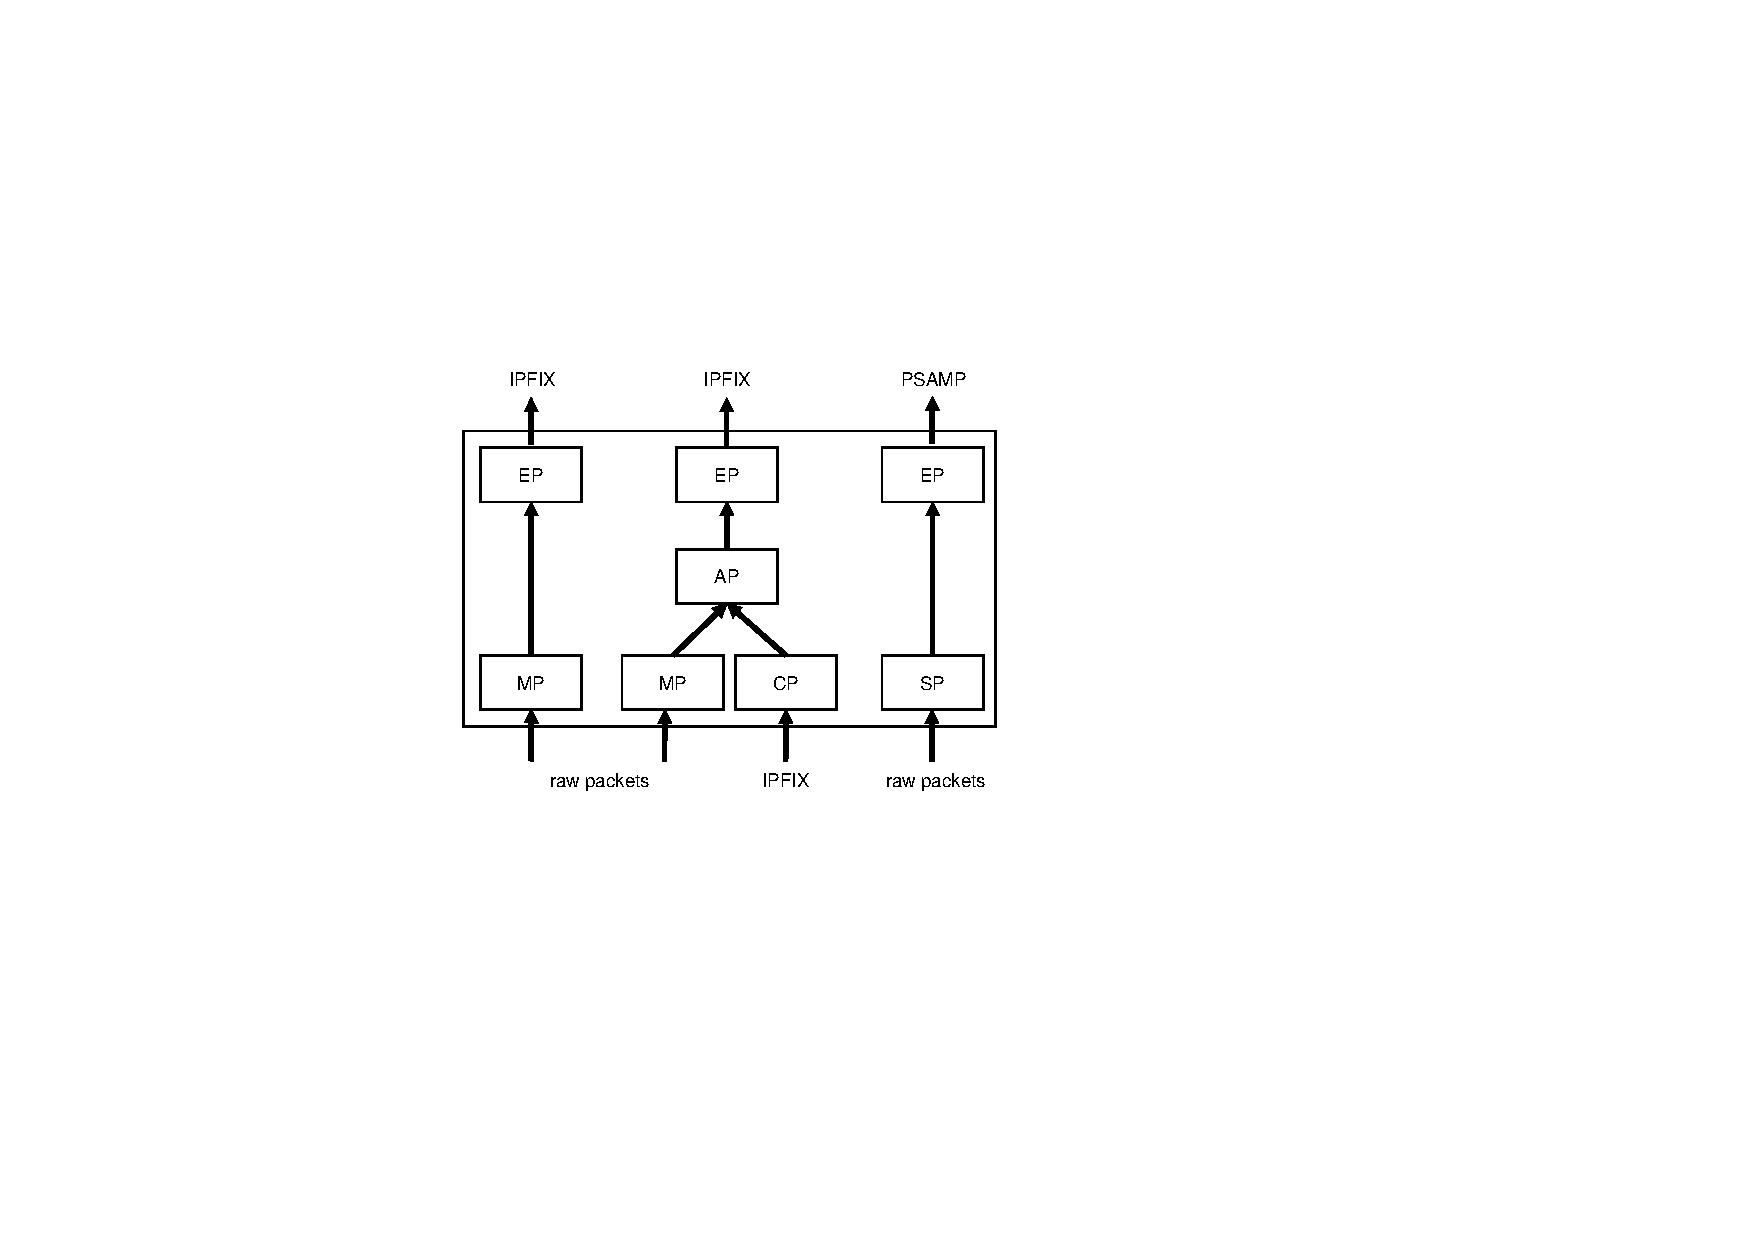
\includegraphics[scale=0.65]{gfx/ipfix-arch3.pdf}
\caption{IPFIX Device Architecture: Metering, collecting and sampling processes feed data to aggregation and exporting processes}
\label{fig_ipfix_arch}
\end{center}
\end{figure}


In this paper, we present the monitoring toolkit Vermont, which has been developed in the \emph{History} project~\cite{dressler2005history} and the European project \emph{Diadem Firewall}.
Vermont was designed for monitoring high-speed networks with link speeds of up to one gigabit per second using standard PC hardware.
Furthermore, Vermont serves as a reference implementation of the aforementioned monitoring techniques, including the protocol extensions for flow aggregation~\cite{dressler-ipfix-aggregation}.

The design principles of Vermont are:
\begin{itemize}
\item IPFIX/PSAMP compliant monitoring and data export
\item Rule-based flow metering and aggregation
\item Hardware-independent packet capturing
%\item Efficient, decoupled data processing
\item Multiprocessor support
\item High monitoring performance
\end{itemize}

The remainder of this paper is organized as follows.
Section~\ref{sec:related-work} briefly introduces other open-source implementations of monitoring probes and compares them to Vermont.
Section~\ref{sec:architecture} outlines Vermont's architecture.
Application scenarios are provided in section~\ref{sec:scenarios} and results obtained in performance, compatibility, and robustness evaluations are discussed in section~\ref{sec:evaluation}.
Finally, section~\ref{sec:conclusion} concludes the paper.


\section{Related Work}
\label{sec:related-work}

%Network monitoring tools have a long history in the communications domain. 
%Usually, such approaches were integrated into special-purpose applications for accounting or traffic engineering environments. 
%With the development of the Netflow protocol by Cisco, a standardized method emerged that allows a strict separation of monitoring and analysis. The IETF recognized the need for an Internet-wide standard for collecting and transporting monitoring data. Therefore, NetFlow.v9, IPFIX and PSAMP are being standardized as RFCs.

In this section, we provide a brief overview to open-source implementations of monitoring probes.
There are several implementations supporting the NetFlow.v9 format, e.g. nprobe~\cite{deri2003nprobe} and NetMate~\cite{schmoll2004netmate}. Currently, the authors of these tools are working on IPFIX compliant versions.
Table~\ref{tab:features} compares the supported features of these implementations and Vermont.
%Futher, there exist implementations at Cisco Systems and IBM~\cite{ibm-ipfix} which are not available under an open-source compatible license and as such not listed here.

Vermont, being a reference implementation for both the IPFIX and the PSAMP standard, already supports IPFIX, PSAMP, and IPFIX aggregation schemes.

\begin{table}
%% increase table row spacing, adjust to taste
\renewcommand{\arraystretch}{1.0}
\caption{Feature Comparision}
\label{tab:features}
\begin{center}
%% Some packages, such as MDW tools, offer better commands for making tables
%% than the plain LaTeX2e tabular which is used here.
\begin{tabular}{r|c|c|c}
 & Vermont & nProbe & NetMate\\
\hline
IPFIX Support & yes & planned & \\
PSAMP Support & yes &  & \\
IPFIX Aggregation & yes & planned & planned\\
Collector Functionality & yes &  & \\
Save Data To Disk &  & yes & \\
Save Data To SQL DB & yes & & \\
Remote Reconfigurability & yes &  & yes\\
Plugin Architecture &  & yes & yes\\
\hline
\end{tabular}
\end{center}
\end{table}



\section{Architecture}
\label{sec:architecture}

\subsection{Overview}

Figure~\ref{fig_allmodules} depicts the architecture of Vermont.
The functionality is divided into two main modules: A sampler module and a concentrator module.
The sampler module implements all packet-based functions like packet capturing, filtering, sampling and PSAMP export.
The functions for flow accounting and aggregation are provided by the concentrator module.
Both main modules can run independently or in combination; in the second case, the sampled packets are passed from the sampler module to the flow metering and aggregation function of the concentrator module.
A common exporter library called ipfixlolib realizes the export of monitoring data using the IPFIX/PSAMP protocol.

Both main modules are broken up into submodules, which are described in the following subsections.
The main modules, as well as their submodules, have been designed for being instantiated more than once, giving the user a maximum degree of flexibility and caring for a wide range of monitoring needs.
This modular approach also guarantees a high level of reusability and eases the incorporation of selected components into other software packages.

Vermont's modular design excells where customization is needed. Implementing the SQL database writer was a matter of simply writing an alternative export module and changing Vermont's configuration routines so it could be instantiated when configured to. A base class takes care of the details like allocating buffered queues and two methods \texttt{run()} and \texttt{terminate()} have to be implemented which start and shutdown the module's operation.
We use an URI-based scheme to indicate the export method used, i.e. exporting to the host \texttt{10.20.30.40} with destination port 6677 using the UDP protocol is expressed by \texttt{udp://10.20.30.40:6677}. This scheme can be arbitrarily extended.

%Internally, each of Vermont's three main functions - capturing, filtering and exporting - is contained within its own thread.
%Forwarding data between subsystems is done by putting references to the actual data into buffered queues connecting the subsystems.
%This design was chosen to fully exploit multi-processor-systems and, ultimately, aid scalability by allowing asynchronous processing while avoiding unnecessary copying or locking of data.
Internally, submodules are contained within different threads.
In order to avoid unnecessary copying of data, only references to the actual data are passed from one subsystem to the other using buffered queues.
This design was chosen to optimally exploit the asynchronous processing capabilities of multi-processor systems.

Vermont's configuration is maintained in one consistent configuration file; additionally, a back-end for dynamic reconfiguration using Netconf protocol has been implemented~\cite{muenz2006using}, allowing for fast remote distribution of new configuration data.

Depending on the configuration, Vermont captures raw packets, performs packet sampling and optional flow accounting and exports the resulting monitoring data using the IPFIX/PSAMP protocol.
Alternatively, Vermont can operate as an IPFIX concentrator that receives and aggregates data exported by other monitoring probes in order to reduce the overall data volume.


\begin{figure}
\begin{center}
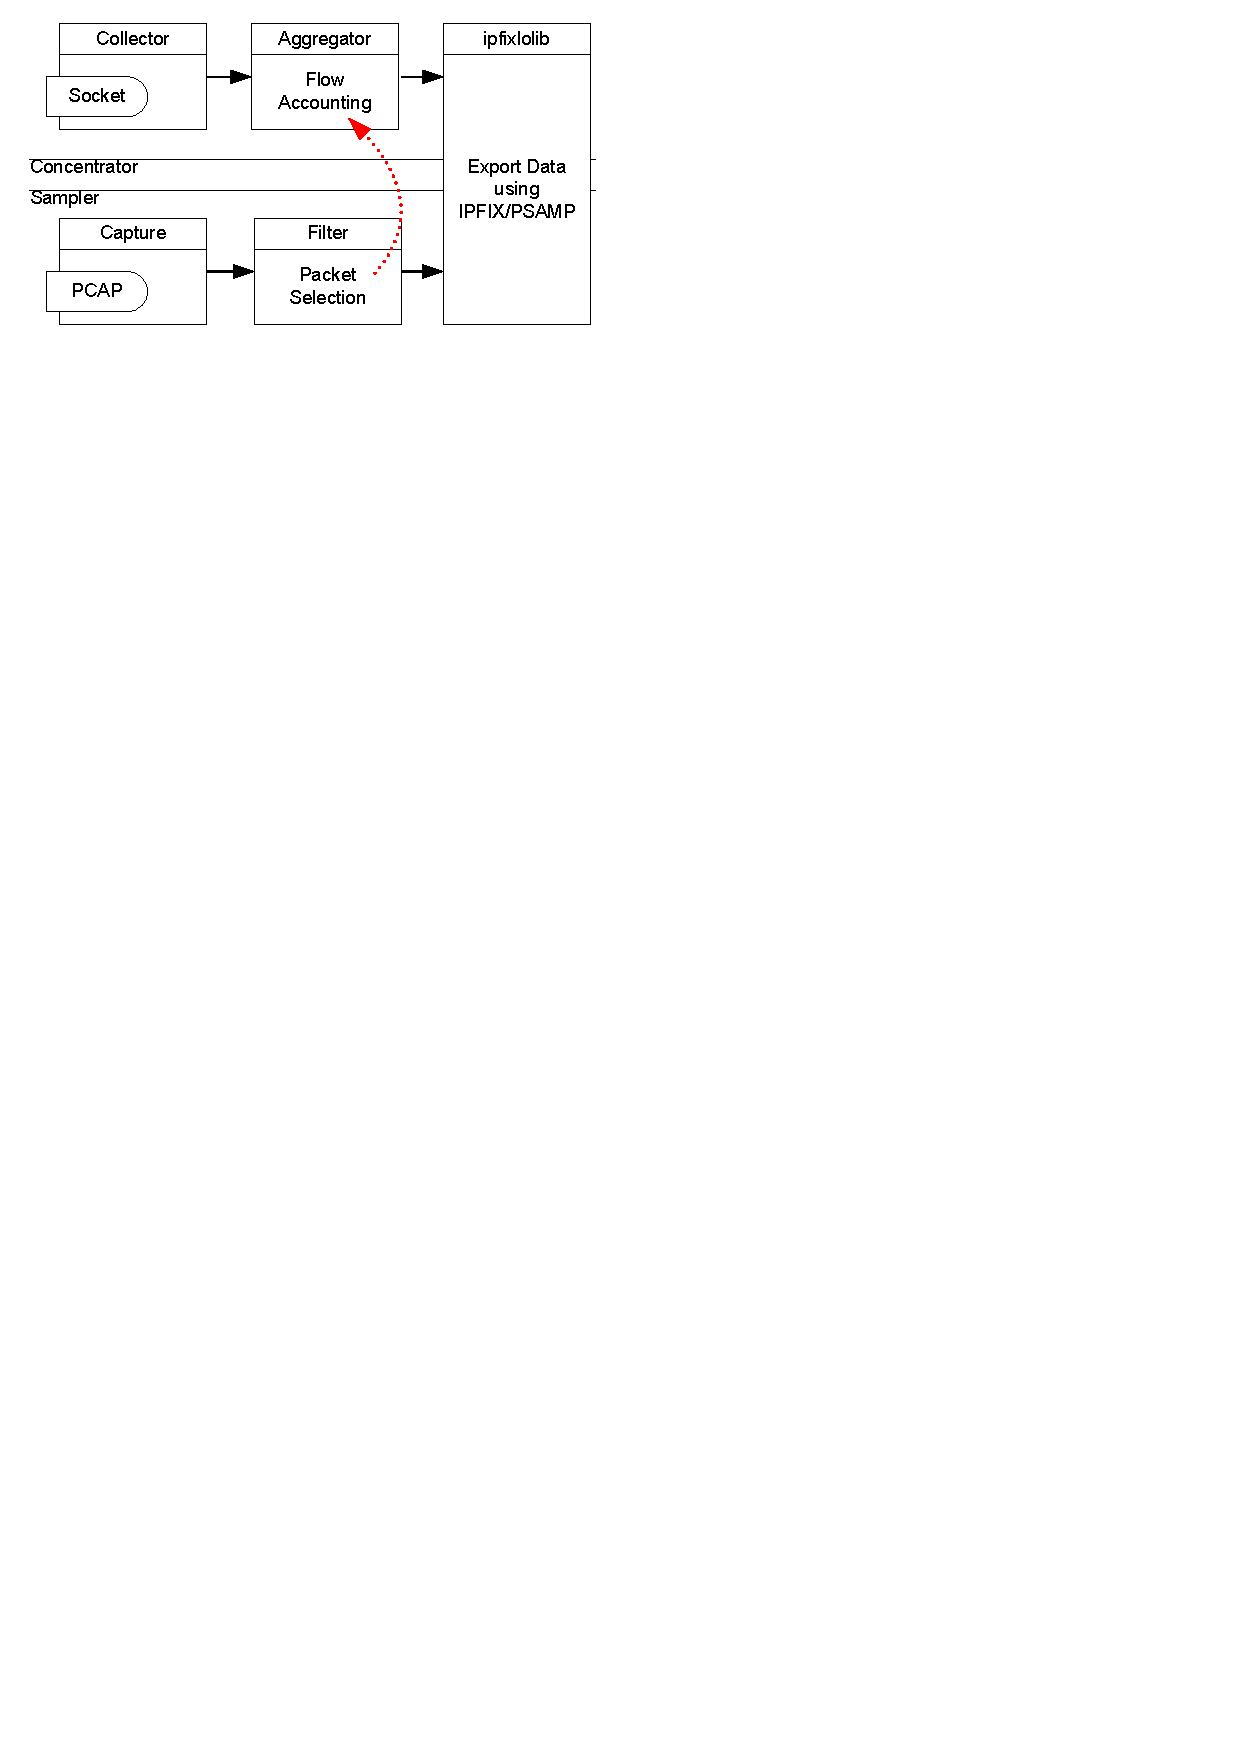
\includegraphics[scale=0.65]{gfx/vermont-arch2.pdf}
\caption{Vermont: Architectural overview}
\label{fig_allmodules}
\end{center}
\end{figure}


\subsection{Sampler Module}
\label{sec_sampler}

The sampler module captures raw packets from network interfaces, selects individual packets based on filters and sampling algorithms as specified in~\cite{ietf-psamp-sample-tech} and exports the resulting data.
Filters and sampling algorithms are implemented as packet processors that can be executed in arbitrary order.
% that provide all fields required by the configured templates
Non-matching packets or packets that are sorted out by a sampling algorithm are immediately dropped and only packets that have passed all packet processors are exported.
At any point in the packet processor chain, packets can also be injected into the concentrator module to be processed by the flow metering and aggregation function.

\subsection{Concentrator Module}
\label{sec_concentrator}

Vermont's concentrator module consists of a NetFlow.v9/IPFIX collector, an aggregator and an IPFIX exporter, all interconnected using callbacks.
The aggregator submodule implements the rule-based flow metering and aggregation approach specified in~\cite{dressler-ipfix-aggregation}.
It can be configured to process flows received via the IPFIX collector and/or packets injected by the sampler module; this is shown in figure~\ref{fig_allmodules} by the dotted arrow.
That way, the aggregator can be deployed for flow accounting of local traffic as well as for concentration of flow records received from other monitoring probes. 


%\subsection{ipfixlolib}
%\label{sec_ipfixlolib}
%
%Both subsystems export their data using a library aiding the sending of IPFIX/PSAMP-encoded data.
%It provides a C API with the following functionalities:
%\begin{itemize}
%\item conversion of IPFIX identifiers into their numerical representation et vice versa
%%\item automatic conversion of data and meta-data from HBO to NBO et vice versa
%\item protocol-compliant periodic export of templates
%\item export of metering data to one or several collectors
%\end{itemize}


\section{Monitoring Scenarios}
\label{sec:scenarios}

% "some of which" sounds really nice -RLA
Owing to the flexibility offered by its modular design, Vermont can be used in a wide range of scenarios, some of which are presented in this section. Data export can be done to one or more collecting stations.

\subsection{PSAMP Probe}
With only the sampler module activated, Vermont acts as a PSAMP probe that captures packets from network interfaces, selects individual packets based on filters and sampling algorithms and exports the resulting packet-based monitoring data.

\subsection{IPFIX Probe}
In this mode, Vermont performs rule-based flow accounting~\cite{dressler-ipfix-aggregation} on locally observed packets. Both the sampler module and the concentrator module are activated.
The sampler module is configured to pass packets to the concentrator module, which performs flow accounting and exports the resulting flow records. For example, flow accounting can be used to generate byte or packet counters for the observed network.
The sampler module's exporter, as well as the concentrator module's collector, are disabled.

\subsection{Concentrator}
Only the concentrator module is activated. Flow records from other monitoring probes are received at the collector. Rule-based flow aggregation~\cite{dressler-ipfix-aggregation} is performed in order to reduce the amount of monitoring data.
The resulting records are exported to higher-level concentrators or traffic analyzers.

\subsection{Specific accounting for SYN flood detection}
In the context of \emph{Diadem Firewall}, Vermont is used to count TCP SYN and SYN/ACK packets. The resulting counter values are used to detect SYN flood attacks on protected servers using the SYN-dog algorithm~\cite{wang02syndog}.



\section{Evaluation}
\label{sec:evaluation}

Vermont and its modules have undergone extensive testing with respect to performance, interoperability and robustness.

\subsection{Performance}

Figure~\ref{fig_perf_sampler} shows the results obtained from benchmarking the sampler module on a dual-processor system\footnote{Dual 3.06GHz Intel Xeon, 2GB RAM, 1GBit NIC, Linux Kernel 2.6.13, libpcap-mmap 0.9.20060417}.
A specialized version~\cite{pcap-mmap} of the pcap library was used, which avoids multiple copying of captured data by mapping a user-space buffer into the kernel.
The traffic was generated using a packet generator set to fixed packet generation rates running on a seperate machine. To ensure the desired packet rates the UDP protocol was used 
%and the observed rate fluctuation averaged at 1.4\%.
and every two seconds captured as well as dropped packets were accounted using the counters supplied by the pcap library. Multiple tests have proven the data sample shown in figure~\ref{fig_perf_sampler} to be Vermont's typical behaviour over time.

Until a packet rate of 250,000 packets per second (for 128 byte packets), the capture rate is 100\%.
420,000 packets per second denotes the maximum packet generation rate and short-lived loss up to 45 percent can be observed; however, the loss is not of permanent nature and numerous measure points suggest the packet loss ratio being substantially smaller, averaging at 9.0 percent. At 300,000 packets per second the loss averages at 3.8 percent.
The diagram shows a certain fluctuation regarding the packet capture ratio. This stems from Vermont's asynchronous design utilizing buffered queues between subsystems. If the input queue suffers from congestion incoming packets will no longer be forwarded, but immediately dropped instead.
Capturing entire packets of 1500 bytes in size showed no loss at a maximum observed rate of 60,000 packets per second.

\begin{figure}
\begin{center}
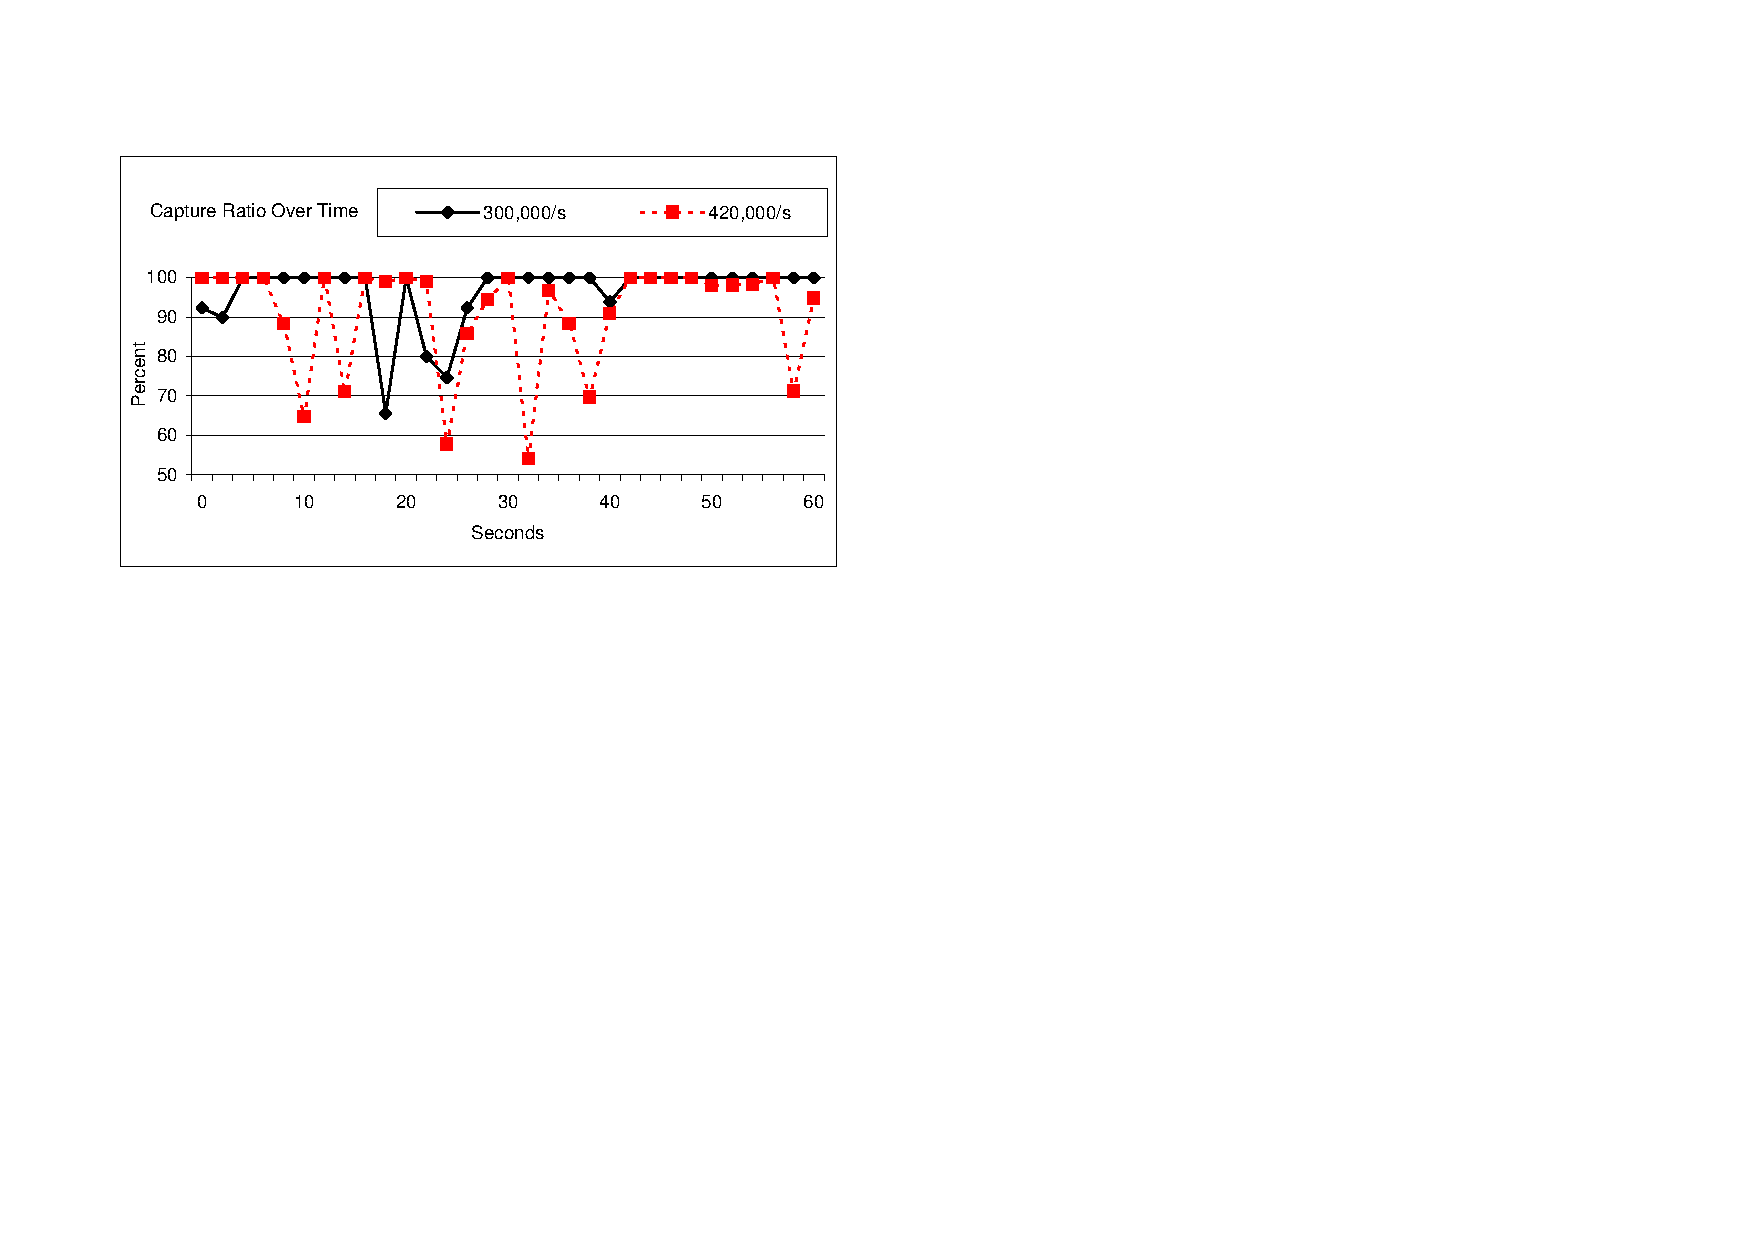
\includegraphics[scale=0.7]{gfx/sampler-perf3.pdf}
\caption{Capture ratio for packet rates of 300,000 and 420,000 packets per second}
\label{fig_perf_sampler}
\end{center}
\end{figure}

The concentrator module's performance was tested in a real-world scenario.
Vermont was configured to capture all packets at the access router of our university's network, perform flow accounting using the rules shown in figure~\ref{fig_rule} and export the resulting records.
FIXME These rules create aggregated fields for packet and byte counters.
During the tests, a maximum metering performance of 45,000 flows per second was achieved\footnote{Dual 2.0GHz Intel Xeon, 1GB RAM, 1GBit NIC, Linux Kernel 2.6.13, libpcap-mmap 1.0.20050129}. 
Repeating the test with different rule sets showed the maximum number of metered flows to be inversely proportional to the number of rules.

\begin{figure}
\centering
\fbox{\begin{minipage}{7cm}
\scriptsize{\texttt {keep protocolIdentifier\\
keep sourcetransportport\\
keep sourceipv4address\\
keep destinationtransportport\\
keep destinationipv4address\\
aggregate inpacketdeltacount\\
aggregate inoctetdeltacount\\
aggregate flowcreationtime\\
aggregate flowendtime}
}
\end{minipage}}
\caption{Aggregation rule used by Concentrator module}
\label{fig_rule}
\end{figure}


\subsection{Interoperability and Robustness}

We participated in the IST MOME IPFIX Interoperability testing event~\cite{mome-interop} in July 2005 and tested Vermont's interoperability with several other IPFIX/PSAMP implementations. 
Vermont's collector and exporter successfully passed all applicable tests, including the handling of corrupt IPFIX data packets and showed excellent robustness and compatibility.





\section{Conclusion}
\label{sec:conclusion}

In this paper, we presented Vermont, a monitoring toolkit for flow monitoring and packet sampling.
Vermont has fulfilled its design goal of providing a versatile high-speed monitoring toolkit consisting of a modular, reusable, and freely configurable architecture. Excellent compatibility and high robustness have been proven in interoperability tests.
Vermont is available as an open-source package~\cite{vermont-site}.


% use section* for acknowledgement
\section*{Acknowledgment}
We gratefully acknowledge support from the European project \emph{Diadem Firewall} (FP6 IST-2002-002154). 
Furthermore, we would like to thank Jan Petranek, Michael Dr\"uing, and Lothar Braun for contributing to the development of Vermont.





% Reminder: the "draftcls" or "draftclsnofoot", not "draft", class option
% should be used if it is desired that the figures are to be displayed while
% in draft mode.

% An example of a floating figure using the graphicx package.
% Note that \label must occur AFTER (or within) \caption.
% For figures, \caption should occur after the \includegraphics.
%
%\begin{figure}
%\centering
%\includegraphics[width=2.5in]{myfigure}
% where an .eps filename suffix will be assumed under latex, 
% and a .pdf suffix will be assumed for pdflatex
%\caption{Simulation Results}
%\label{fig_sim}
%\end{figure}


% An example of a double column floating figure using two subfigures.
%(The subfigure.sty package must be loaded for this to work.)
% The subfigure \label commands are set within each subfigure command, the
% \label for the overall fgure must come after \caption.
% \hfil must be used as a separator to get equal spacing
%
%\begin{figure*}
%\centerline{\subfigure[Case I]{\includegraphics[width=2.5in]{subfigcase1}
% where an .eps filename suffix will be assumed under latex, 
% and a .pdf suffix will be assumed for pdflatex
%\label{fig_first_case}}
%\hfil
%\subfigure[Case II]{\includegraphics[width=2.5in]{subfigcase2}
% where an .eps filename suffix will be assumed under latex, 
% and a .pdf suffix will be assumed for pdflatex
%\label{fig_second_case}}}
%\caption{Simulation results}
%\label{fig_sim}
%\end{figure*}



% An example of a floating table. Note that, for IEEE style tables, the 
% \caption command should come BEFORE the table. Table text will default to
% \footnotesize as IEEE normally uses this smaller font for tables.
% The \label must come after \caption as always.
%
%\begin{table}
%% increase table row spacing, adjust to taste
%\renewcommand{\arraystretch}{1.3}
%\caption{An Example of a Table}
%\label{table_example}
%\begin{center}
%% Some packages, such as MDW tools, offer better commands for making tables
%% than the plain LaTeX2e tabular which is used here.
%\begin{tabular}{|c||c|}
%\hline
%One & Two\\
%\hline
%Three & Four\\
%\hline
%\end{tabular}
%\end{center}
%\end{table}



% trigger a \newpage just before the given reference
% number - used to balance the columns on the last page
% adjust value as needed - may need to be readjusted if
% the document is modified later
%\IEEEtriggeratref{8}
% The "triggered" command can be changed if desired:
%\IEEEtriggercmd{\enlargethispage{-5in}}

\bibliographystyle{IEEEtran}
\bibliography{vermont-paper}

\end{document}


